%\documentclass{svjour3}                     % onecolumn (standard format)
%\documentclass[smallcondensed]{svjour3}     % onecolumn (ditto)
\documentclass[smallextended, natbib]{svjour3}       % onecolumn (second format)
%\documentclass[twocolumn]{svjour3}          % twocolumn
%
\smartqed  % flush right qed marks, e.g. at end of proof
%
\usepackage{graphicx}
%\usepackage{cite},
\usepackage{amsmath}
\usepackage{mathptmx}  
\usepackage{subfigure}    % use Times fonts if available on your TeX system
%\usepackage{natbib}
%
% insert here the call for the packages your document requires
%\usepackage{latexsym}
% etc.
%
% please place your own definitions here and don't use \def but
% \newcommand{}{}
%B
% Insert the name of "your journal" with
% \journalname{myjournal}
%
\begin{document}

\title{The Alejandro Project: Testing the Target Contrast Signal Theory\thanks{ESRC grant?}
}
\subtitle{Replication and Generalisation}

\titlerunning{Testing the TCS Theory}        % if too long for running head

\author{Anna Hughes \and Anna Nowakowska \and Alasdair D. F. Clarke}

%\authorrunning{Short form of author list} % if too long for running head

\institute{F. Author \at
              first address \\
              Tel.: +123-45-678910\\
              Fax: +123-45-678910\\
              \email{fauthor@example.com}           %  \\
%             \emph{Present address:} of F. Author  %  if needed
           \and
           S. Author \at
              second address
}

\date{Received: date / Accepted: date}
% The correct dates will be entered by the editor

\maketitle

\begin{abstract}
Insert your abstract here. Include keywords, PACS and mathematical
subject classification numbers as needed.
\keywords{First keyword \and Second keyword \and More}
% \PACS{PACS code1 \and PACS code2 \and more}
% \subclass{MSC code1 \and MSC code2 \and more}
\end{abstract}

\section{Introduction}
\label{intro}

\paragraph{Background}
Visual search, where participants are asked to find a target within a cluttered scene, has been extensively studied within psychology. Several models have been developed that can generate testable predictions about how different types of distractors and targets affect search efficiency.

The two most studied families of models of visual search include bottom-up models (also known as visual saliency models) and top-down models. Saliency models rest on the assumption that fixations are directed to objects or locations that are most dissimilar to the background or other objects in the visual display \cite{itti2000saliency, itti1998model, koch1987shifts}. While the original saliency model was able to predict fixation allocation in a visual search task above chance \cite{parkhurst2002modeling}, further research demonstrated that a comparable level of performance could be achieved using a simple central fixation bias heuristic \cite{tatler2007central}. The saliency models have since been extended and improved (see for example \cite{zhang2008sun}): however, the main issue with this family of models remains their limited usability in complex real-life search arrays \cite{tatler2011eye, koehler2014saliency}. In addition, in most instances of visual search, the target is clearly defined (i.e. the goal is to find a specific object) and inspecting the most salient areas of the display may in these cases be inefficient.

Another class of models are based around Feature Integration Theory \cite{treisman1980feature}, which has been modified and extended by Wolfe in the Guided Search Model \cite{wolfe1989guided,wolfe2014approaches}. These models combine top-down influences (how closely an item resembles the observer's goal) with bottom-up image properties. For example, if one's goal (top-down processing) is to find a red horizontal bar, all the red and horizontal items in a visual search display will be given greater weight than distractors (e.g. vertical and blue items) in the model. The salience of a given object in the display (how distinctive it is from the surrounding objects) also activates bottom-up processing. For instance, a blue item among red items is ranked higher than red among orange items. Combining bottom-up and top-down sources of activation generates an activation map which generates a prediction of the order in which stimuli are processed in visual search. Thus, these models aim to produce a representation of the visual properties of the distractors at each location in the visual field. 
 
However, more recent work has taken a different approach, focusing solely on representing the difference between targets and distractors. For example, in work on eye movement patterns, it has been proposed that performance in inefficient (serial) visual search is mostly determined by the size of the 'functional viewing field', whose size varies as a function of target-distractor similarity \cite{hulleman2017brink}. One recent model, the Target Contrast Signal (TCS) Theory \cite{lleras2020target} aims to provide a unifying, quantitative framework that can make behavioural predictions based on this general assumption.

\paragraph{Theoretical intro to TCS}
TCS proposes that behaviour is determined by comparing the target template (held in memory) with every element present in the scene in parallel. This allows the visual system to reject peripheral non-targets quickly; the speed at which items are evaluated is determined by how different the item is from the template through an evidence accumulation process (formally, the slope of the logarithmic function is assumed to be inversely proportional to the overall magnitude of the contrast signal between the target and distractor). The model thus focuses on an initial, efficient processing stage of search; if sufficient evidence is not accumulated during this process, the model posits that a second stage is entered, where attention is deployed serially. TCS has been successful in predicting a number of empirical results, including search performance in heterogeneous scenes based on parameters estimated in homogeneous scenes, both with artificial stimuli \cite{buetti2016towards,lleras2019predicting} and with real-world objects visualised on a computer display \cite{wang2017predicting}. 
 
\paragraph{Limitations, and extending basic stimuli} While results to date for TCS appear promising, they remain relatively preliminary, being tested by only one research group so far. There remains a great deal of scope for extending beyond the parameters tested to date (such as the number of distractors) in order to test the robustness and generalisability of the model. In addition, there are some predictions of the model, including its ability to explain search asymmetries, that have yet to be empirically confirmed \cite{lleras2020target}.

\paragraph{Within subjects}
In addition, in all implementations of TCS so far, predictions of search efficiency (e.g. in heterogeneous scenes) have been made on the average of a group of participants, using data from a different group performing a different task (e.g. searching in homogeneous scenes). Thus, we know that TCS can replicate group-level averages between subjects in search well, but we do not know whether it is also able to make predictions at the individual level. This is particularly important given that conclusions based on aggregate data can be different from those that take individual differences into account; in one study where participants searched for a target in an array of randomly oriented line segments, aggregating the data suggested that participants were using a stochastic search model. However, when considering each participant individually, it became clear that there was a high level of heterogeneity in responses, with some participants performing close to optimally, and others actually performing worse than chance \cite{nowakowska2017human}. Similarly striking variability has also been reported in other search studies \cite{irons2016choosing, irons2018characterizing}. 

\paragraph{Conclusion to introduction} 
In the current manuscript, we focus on replicating and extending findings from \cite{buetti2019predicting}. Here, participants searched for a target in a scene of homogeneous distractors. First, parallel search efficiency (measured by the logarithmic search slope) was estimated for cases where the distractors varied from the target in one dimension: either colour (e.g. a cyan target being searched for in either yellow, blue or orange distractors) or shape (e.g. a semicircle target in either circle, diamond or triangle distractors). New participants then searched for the same targets in displays where the distractors were compounds, differing from the target in both colour and shape (e.g. searching for a cyan semicircle in either blue circles, orange diamonds or yellow triangles). Figure \ref{fig:buetti2019_stimulus} shows example stimuli from their paper. The logarithmic search slopes in the initial experiments were then used to predict the logarithmic slopes and reaction times using a number of models. The authors found that the best model was a 'collinear contrast integration model' where the distinctiveness scores were summed along each attribute in the unidimensional experiments, creating an overall contrast score that was used for compound stimuli predictions.

\begin{figure}
\centering
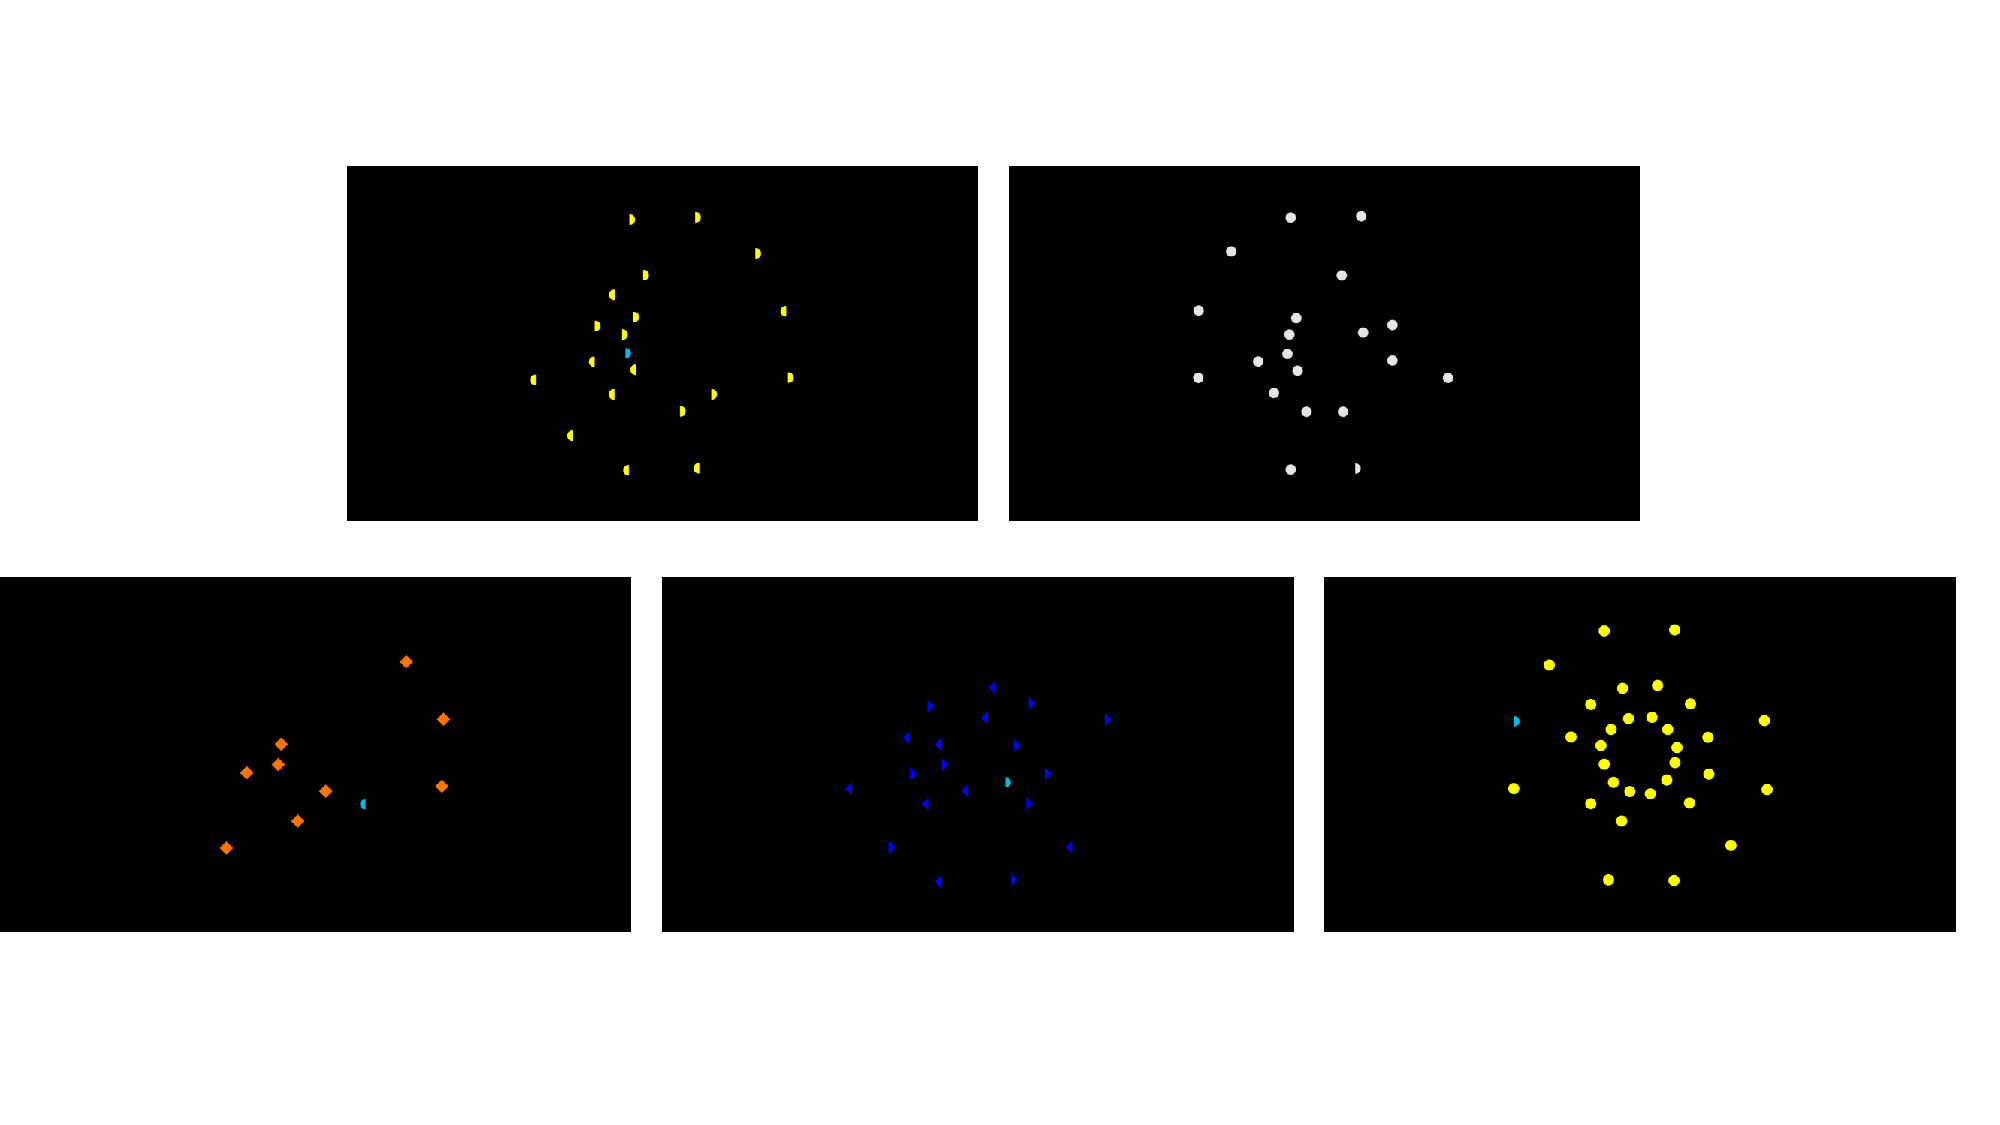
\includegraphics[width=\textwidth]{../plots/example_stimuli_figure.pdf}
\caption{Example stimuli from \cite{buetti2019predicting} Top left: Expt 1A. Here, the target is a blue semicircle within a set of homogeneous (yellow semicircle) distractors. Top right: Expt 1B. The target is a grey semicircle in circular grey distractors. Bottom left: Expt 2A. The target is a blue semicircle in orange diamond distractors. Bottom middle: Expt 2B. The target is a blue semicircle in dark blue triangle distractors. Bottom right: Expt 2C. The target is a blue semicircle in yellow circular distractors.}
\label{fig:buetti2019_stimulus}
\end{figure}

\paragraph{Overview of the current study}
We first run a replication of \cite{buetti2019predicting}, in an online, within-subjects study. This design allows us to extend the modelling, both incorporating a multi-level design to predict within-subjects effects and by utilising a Bayesian generalised linear model framework to better represent the distribution of responses (e.g. avoiding predicting negative reaction times, accounting for uncertainty in model predictions). We  also carry out a direct analytical replication using the same methods as in \cite{buetti2019predicting} allowing us to ask whether the choice of analysis affects the results.

\section{The Target Contrast Model}
\label{sec:reansalysis}

We first describe the original Target Contrast Model (and verify that we can replicate the original analysis - see Supplementary Materials). This is followed by our proposed extension.

\subsection{TCS modelling overview} 

In Experiment 1a of \cite{buetti2019predicting}, participants searched for a cyan semicircle target among blue, yellow or orange semicircular distractors i.e. they searched for a target that differed from the distractors by a \textit{single feature} (colour). The experiment was then repeated (1b) using a different single feature (shape, with participants searching for the semicircular target within triangle, circle or diamond distractors). In Experiments 2a, 2b and 2c, participants again searched for a cyan semicircle, but this time, the distractors differed in both shape and colour. We will refer to these conditions as \textit{double features}. Note, unlike in standard conjunction searches, in this paradigm, the distractors are all identical with respect to these features (i.e, orange triangles). 

The \textit{Target Signal Contrast} theory allows us to predict the value of the logarithmic slope, $D_\text{c,s}$, in this condition based on the  corresponding $D_j$ in the single feature seach experiments. 

\subsubsection{Calculating the logarithmic slope parameter, $D_i$}
\label{sec:fitting_D}

Experiments 1a and 1b (referred to jointly as Experiment 1) were used to calculate the logarithmic slope parameter $D_i$. In both experiments, the number of distractors varied, allowing the data to be used to fit a log-linear model for reaction times, where reaction times increase linearly with $\log(N_T)$ (the log of the number of distractors) \ref{eq:loglin}. In the original model the error distribution was assumed to be normal. 

\begin{equation}
\hat{RT} = D_i\log(N_T+1) + a
\label{eq:loglin}
\end{equation}

Thus the results of Experiment 1 were used to calculate the logarithmic slope, for each type of distractor. When colour varied, we will refer to $D_c$, for $c=1,2,3$. Similarly for shape we will denote this ($D_s$), and the compound features are denoted as ($D_{c,s}$). As $a$ represented the intercept in our model, it is independent of both shape and colour, as it represents how long observers take to find a target when $N_T = 0$, i.e., there are no distractors.

\subsubsection{Estimating $D_{c,s}$, the logarithmic slope parameter for compound features}

In the context of the current experiments, the core idea of TCS theory is that we can estimate the logarithmic slope parameter for a double feature visual search from the slopes parameters in the two independent single feature searches. I.e., $D_{c,s} = f(D_c, D_s)$.

\cite{buetti2019predicting} tested three different models for predicting $D$ for compound colour-shape stimuli. The best feature guidance model (Equation \ref{eq:bestfeature}) suggests that when the target and lures differ in two dimensions, participants will choose to attend to whichever feature dimension is the most discriminable (i.e. has the smallest $D$ value):

\begin{equation}
D_\text{c,s} = \text{min}\left(D_\text{c}, D_\text{s}\right)
\label{eq:bestfeature}
\end{equation}

The orthogonal contrast combination model instead suggests that independent feature dimensions comprise a multidimensional space, where an object can be described by the overall vector in this space, and thus $\mathrm{D_{overall}}$ can be represented as:

\begin{equation}
D_\text{c,s} = \frac{1}{\sqrt{\frac{1}{(D_\text{c})^2 + (D_\text{s})^2}}}
\label{eq:orthogonalcontrast}
\end{equation}

Note: we had to change this a little to make it match! !!!! *******

Finally, the collinear contrast integration model also assumes independence of feature dimensions, but assumes that while the visual features create a multidimensional space, the contrast between them is unidimensional. As $D$ is assumed to be inversely proportional to contrast, the equation can be written as follows:

\begin{equation}
\frac{1}{D_\text{c,s}} = \frac{1}{D_\text{c}} + \frac{1}{D_\text{s}}
\label{eq:collinearcontrast}
\end{equation}

\cite{buetti2019predicting} found that with their dataset, the collinear contrast integration model was best able to predict their empirical RT results with an $R^2 = 93.27\%$. 

We verified we were able to replicate the results of \cite{buetti2019predicting} using the dataset available on OSF (https://osf.io/f3m24/)\footnote{downloaded on 28th August 2020} and using the exclusion criteria originally applied\footnote{We also applied some additional exlusion crit!}; see \textit{Supplementary Materials} for details. See Figure \ref{fig:comp_rep}(left panel).

\begin{figure}
\centering
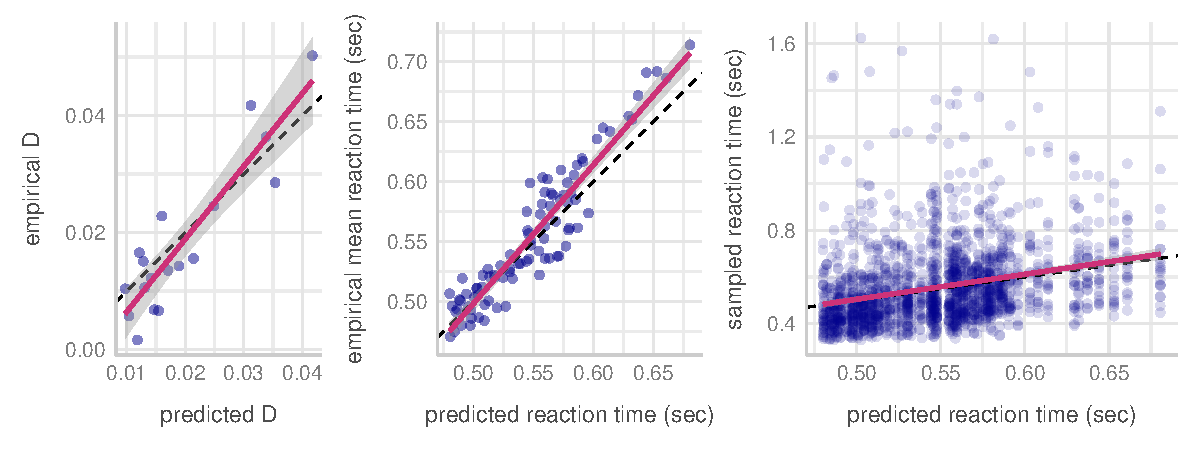
\includegraphics[width=\textwidth]{../plots/computational_replication.pdf}
\caption{(left) The collinear method for calculating $D$ offers a good prediction. (centre) Using the TSC to predict reaction times. (right) Each dot now represents a randomly sampled reaction time from an observer.}
\label{fig:comp_rep}
\end{figure}

\subsubsection{Estimating mean reaction times}

The TCS theory now allows us to predict mean reaction times:

\begin{equation}
RT = D{c,s}\log(N_T+1) + a
\end{equation}

As can be seen in  Figure \ref{fig:comp_rep} (centre panel), these predictions are very close to the observed values. 

\subsubsection{Discussion}

While TCS theory offers a good prediction of search slopes and corresponding mean reaction times for double feature search, there are two related limitations. Firstly, it is unable to account for individual differences between observers, only the changes to the sample average. Secondly, it cannot account for the distribution of reaction times over multiple trials. Figure \ref{fig:comp_rep} (right panel) shows clearly that these factors generate high levels of variability within the individual trial-level data. To address these issues, we propose a second version of the TCS that makes use of multi-level modelling techniques.

\subsection{A multi-level TCS}

Switching from a linear regression model to a multi-level model will allow us to compute $D$ for each participant, while simultaneously estimating the trial-to-trial variance. We also switch from a frequentist to Bayesian framework, as this allows us to naturally account for the uncertainty in the model's predictions.

However, switching from linear regression to a mutli-level model raises the problem of which distribution to use for modelling reaction times. Using a normal distribution is unlikely to be satisfactory, as it is unable to account for the skew frequently seen in reaction time distributions, and also allows the possibility of negative reaction times. We can account for both of these problems by using a log-normal distribution, $\text{rt} ~ \text{lognormal}(\mu, \sigma))$. We will also test whether a slightly more complex extension of this model, the \textit{shifted lognormal} model (which allows the distribution to be offset to the right i.e. mimicking the patterns seen in reaction time data, where valid responses begin at around 100ms) offers any improvement in model fit.

\subsubsection{Calculating the logarithmic slope parameter, $D_i$}

We began in a similar fashion to section \ref{sec:fitting_D}, although this time, we fitted each model three times using a (i) normal, (ii) lognormal, and (iii) shifted lognormal distribution (please see Supplementary Materials for full details of out modelling approach, including prior predictive checks and model fit diagnostics). The three models were compared using leave-one-out cross validation, and the results showed that the shifted-lognormal model (illustrated in Figure \ref{fig:buetti2019_a1}) was given $100\%$ of the weight. Therefore, we used only this model for the rest of the analysis. 

\begin{figure}
\centering
\subfigure{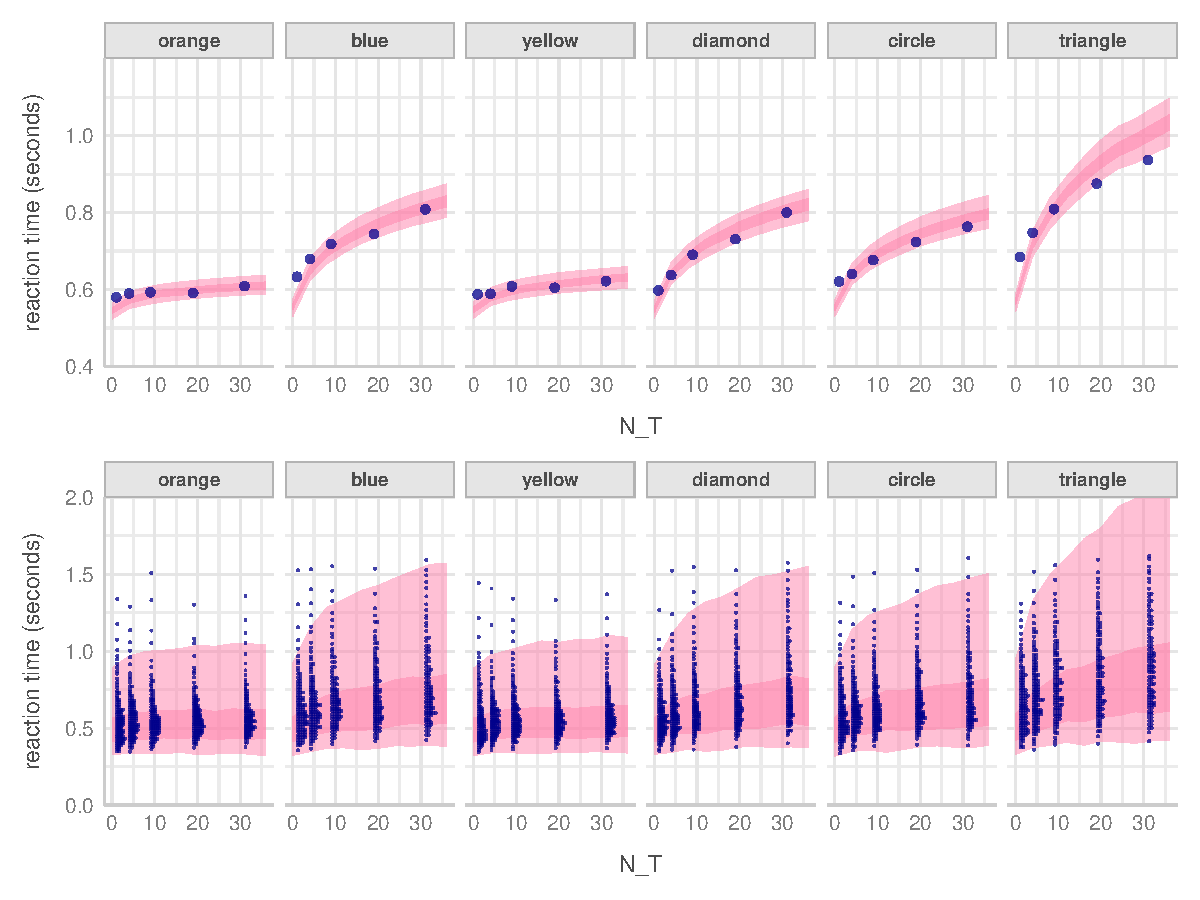
\includegraphics[width=\textwidth]{../plots/bayes_buetti_refit.pdf}}
\caption{(\textit{top}) The shaded regions show the model's estimate ($53\%$ and $97\%$ intervals) of the average participant's mean reaction time, while the points show the empircal mean reaction time. (\textit{bottom}): The shaded regions now indicate the distribution of reaction times (over a new simulated group of participants) generated by the model. The points now represent the 100 quantiles from the empirical data.}
\label{fig:buetti2019_a1}
\end{figure}

We then extracted the posterior distributions for the logarithmic slope parameters as before. The only differences were that i) this approach allowed us to obtain the full posterior distribution for each $D_c$ and $D_s$, rather than just the maximum likelihood fit, and ii) the units are now in $\frac{\log{rt}}{\log{N_T+1}}$ See Figure \ref{fig:buetti2019_D}(bottom).

\begin{figure}
\centering
\subfigure{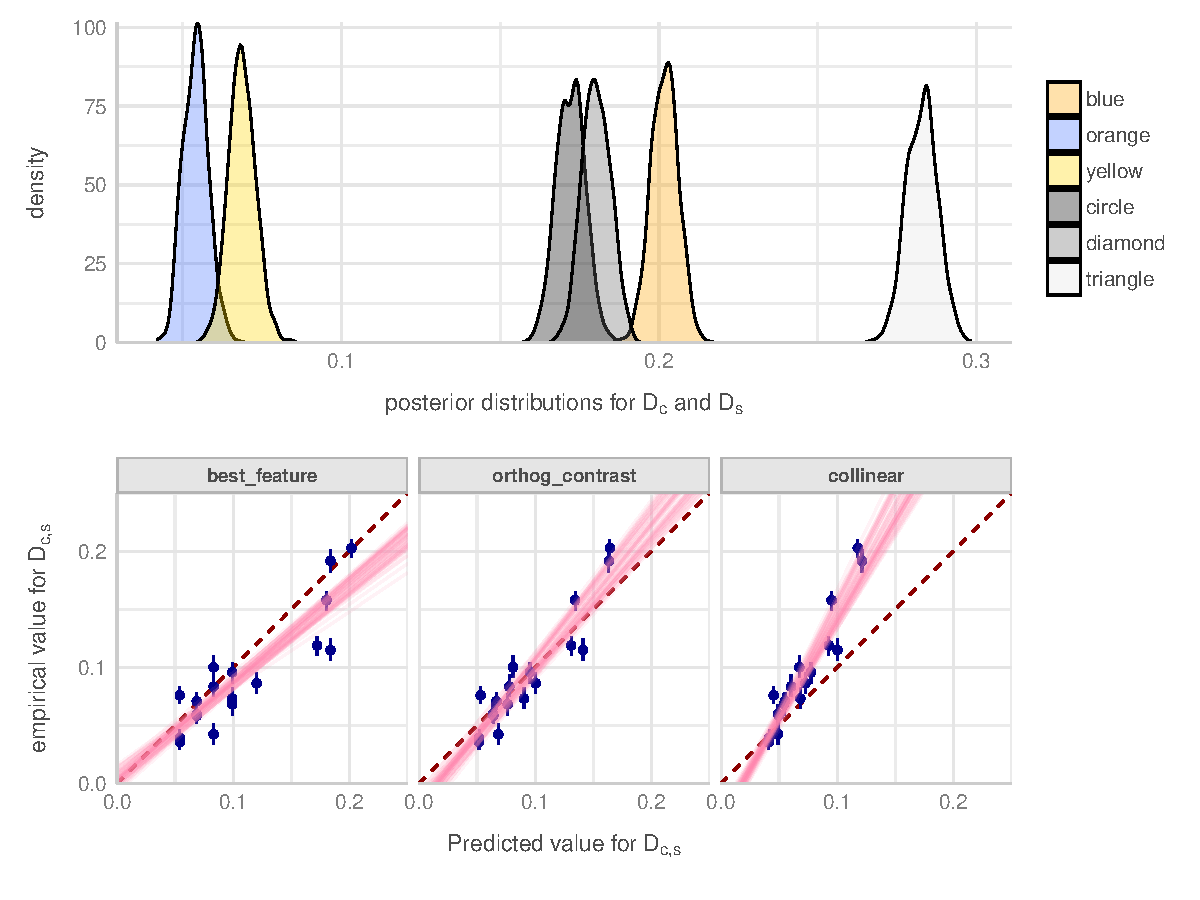
\includegraphics[width=\textwidth]{../plots/bayes_buetti_D.pdf}}
\caption{(\textit{top}) Posterior probability density functions for each $D_c$ and $D_s$ in Experiment 1. As with the original TCS model, when searching for a blue semicircle, triangular distracters are the hardest, while yellow and orange distracters are the eaiest.) (\textit{bottom}) Predicting $D_{c,s}$ from $D_c$ and $D_s$. Crosshairs indicate $97.5$ HPDI for estimates and predictions, while the pink region shows the HDPI for the best fit line. }
\label{fig:buetti2019_D}
\end{figure}

\subsubsection{Estimating $D_{c,s}$, the logarithmic slope parameter for compound features}

We predict $D_{c,s}$ from $D_c$ and $D_c$ in the same way as the original TCS, except this time we use 1000\footnote{check!} samples from the posterior distributions, rather than just the maximum likelihood fit. These predictions are shown in Figure \ref{fig:buetti2019_D}(bottom). We can see that as with the original model, we still find the \textit{best feature} is the worst of the three methods. We additionally calculated a fourth prediction method, the \textit{mean method} which simply takes the averages of the \textit{collinear contrast} and \textit{orthogonal contrast} models.

\subsubsection{Estimating other parameters and predicting reaction times}

Unlike the origianl TCS, before we can use the predicted values of $D_{c,s}$ to generate reaction times, we first have to estimate some additional parameters: 

\begin{itemize}	
\item $\alpha$ - the intercept for the shift\footnote{ndt} parameter.
\item $\phi_a$ - the random intercepts for the linear predictor for $\mu$.
\item $\phi_\alpha$ - the random intercepts for $a$.
\item $\sigma$ - the residual (trial-to-trial) variance. 
\end{itemize}

For the implementation presented here, in order to predict the data from Experiment 2 (4) we will simply use the values for the above parameters obtained from Experiment 1 (3). Once these have been set, we can use the specified model to generate the HDPI intervals for the expected average performance and the full distribution of reaction times over a number of simulated new observers (Figure \ref{fig:buetti2019_rt}).

\begin{figure}
\centering
\subfigure{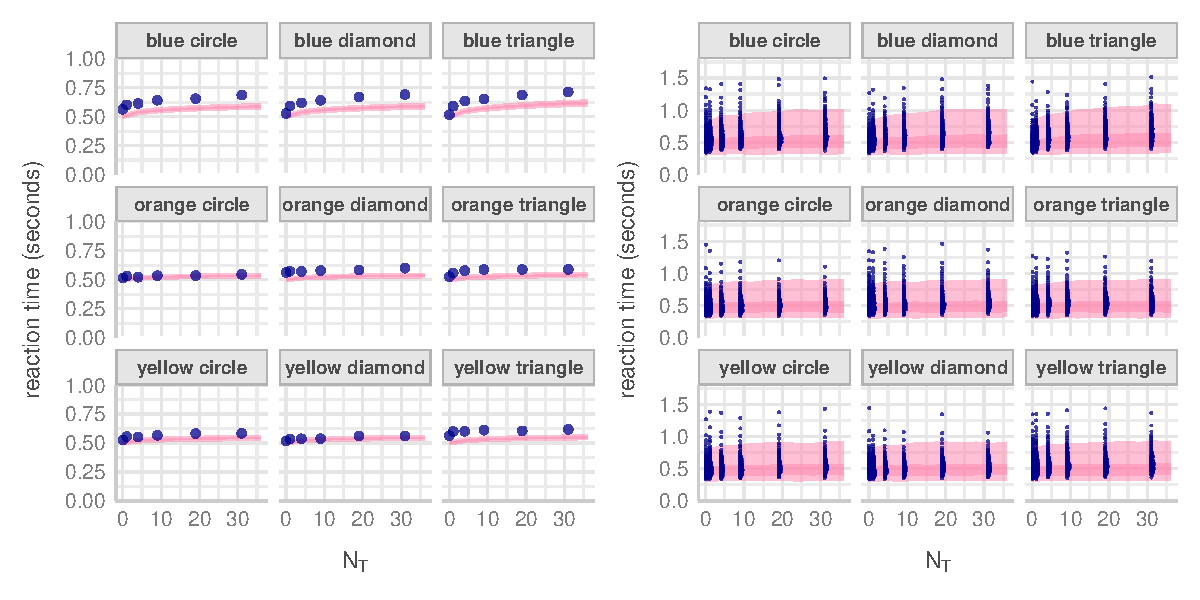
\includegraphics[width=\textwidth]{../plots/bayes_buetti_rt.pdf}}
\caption{(\textit{left}) HDPI and empirical mean reaction times for each condition in Experiment 2. (\textit{right}) Similar, for the full distribution of reaction times over trials. }
\label{fig:buetti2019_rt}
\end{figure}

\subsubsection{Discussion}

Our extension to a multi-level TCS model allows us to go beyond the original version and predict the full distribution of reaction times over samples of known, or new, observers. Moving from a normal to a shifted-lognormal distribution allows us to accuratly model the skew seen in the empirical data, and avoid predicting negative response times. 


\subsection{Discussion}

While we replicate the good predictions using the collinear method if we use a normal distribution, we do not find this that this is the best method if we use a log-normal distribution, and instead, we find the orthogonal contrast method is slightly better. This suggests that (seemingly small) analytical decisions may have important implications for the conclusions drawn. 

\section{Hypotheses}

We plan a number of experiments to test the extent to which the original results in \cite{buetti2019predicting} replicate and generalise. As well as following the original, between-subjects, experiment design, in which data from one group of observers in one task is used to predict behaviour of a second group of participants in a different task, we will allow for within-subject comparisons. Specifically, we will ask: to what extent do the individual differences in the homogeneous task explain the differences in the heterogeneous task? 

\subsection{Registered Hypothesis}

\begin{enumerate}
\item \textbf{Replication of Buetti et al (2019) with online data collection.} Specifically, that the \textit{collinear contrast ingratiation model} outperforms the \textit{best feature guidance}, and \textit{orthogonal contrast combination models}.  Furthermore, the $R^2 = $ ($99\%$ HPDI = $[, ]$) between predicted and observer reaction times.\\
\item \textbf{Larger number of distractors (or targets further in periphery?)} Add an extra ring. Say something about moving from parallel to serial search (although don't use these terms?!!) \\ 
\item Indiv-diff!!!
\item \textbf{Search asymmetries} test O in Qs and Q in Os  ????\\
\end{enumerate}

\subsection{Planned Explorations!}

As these models can be quite challenging to fit, we're making some exucues. But we do plan to use the meothds and framework outlined above (and in suppmat) to more formally investigate the individual differences. We plan to do this by specifying a more complex random effect strucutre, and investigating \ldots

\section{General Methods}

\subsection{Sample Size: Participants and Trials}

Based on the power analysis \ref{sec:power}, we will recruit \ldots

\subsection{Stimuli}

\subsection{Procedure}

\subsection{Data Pre-processing}

incorrect trials? Poorly behaved participants? RTs that are far too short? Or far too long?

\subsection{Analysis Plan}

We will follow the analysis given in Section \ref{sec:reanalysis}.


\section{Experiment 1}



\subsection{Results}
\begin{center}
\textit{-- blank --}
\end{center}

\subsection{Discussion}
\begin{center}
\textit{-- blank --}
\end{center}

\section{Experiment 2}

\subsection{Methods}

Same as Experiment 1? Perhaps we should have a \textit{General Methods} section for both experiments?

\subsection{Results}
\begin{center}
\textit{-- blank --}
\end{center}

\subsection{Discussion}
\begin{center}
\textit{-- blank --}
\end{center}

\section{General Discussion}

Is discriminating between the different models one of our aims? Or is this a discussion point i.e. it's quite hard to do? And therefore maybe a follow up paper?


\begin{acknowledgements}
Thank you to AL for help and encouragement! 
\end{acknowledgements}

% Authors must disclose all relationships or interests that 
% could have direct or potential influence or impart bias on 
% the work: 
%
\section*{Conflict of interest}
The authors declare that they have no conflict of interest.

% BibTeX users please use one of
\bibliographystyle{plainnat}    % basic style, author-year citations
%\bibliographystyle{spmpsci}      % mathematics and physical sciences
%\bibliographystyle{spphys}       % APS-like style for physics
\bibliography{sources}   % name your BibTeX data base

\end{document}